\documentclass[11pt]{article}
\renewcommand{\baselinestretch}{1.5}

\setlength{\oddsidemargin}{-0.1in}
\setlength{\evensidemargin}{-0.1in} 
\setlength{\textwidth}{6.54in}
\setlength{\topmargin}{0in} 
\setlength{\textheight}{8.5in}

\linespread{1}

\usepackage{makeidx}
\usepackage{amsmath,amssymb, amsthm}
\usepackage{latexsym,remreset}
\usepackage[toc,page]{appendix}
\usepackage{graphicx}
\usepackage{multirow}
\usepackage{bbm}
\usepackage{algorithm}
\usepackage{algpseudocode}
%\usepackage[pdftex]{graphicx} 

\usepackage{url}
%% Define a new 'leo' style for the package that will use a smaller font.
\makeatletter
\def\url@leostyle{%
  \@ifundefined{selectfont}{\def\UrlFont{\sf}}{\def\UrlFont{\small\ttfamily}}}
\makeatother
%% Now actually use the newly defined style.
\urlstyle{leo}

\newtheorem{assumption}{Assumption}
\newtheorem{definition}{Definition}
\newtheorem{lemma}{Lemma}
\newtheorem{proposition}{Proposition}
\newtheorem{corollary}{Corollary}
\newtheorem{remark}{Remark}
\newtheorem{theorem}{Theorem}
\newcommand{\mb}[1]{\ensuremath{\boldsymbol{#1}}}
\newcommand{\vol}{{\sf volume}}
\newcommand{\Stochb}{$\Pi_{\mathrm {Stoch}}(b)$}
\newcommand{\tf}{\text{translation factor}}

\title{ISyE6669 HW 5}
\author{}
\date{Spring 2025}

\begin{document}
\maketitle



\begin{enumerate}

\item Compute the gradient $\nabla f(x)$ and Hessian $\nabla^2 f(x)$ of the function
    \begin{align*}
        f(x_1, x_2) = (2x_1 + x_2^2 - 4)^2 + (x_1^2 + x_2 - 8)^2.
    \end{align*}

\subsection*{Solution.}

First, we compute the gradient $\nabla f(x)$ of the function $f(x_1, x_2) = (2x_1 + x_2^2 - 4)^2 + (x_1^2 + x_2 - 8)^2$.

We perform partial differentiation for each component:

\begin{align}
\frac{\partial f}{\partial x_1} &= 2(2x_1 + x_2^2 - 4) \cdot 2 + 2(x_1^2 + x_2 - 8) \cdot 2x_1 \\
&= 4(2x_1 + x_2^2 - 4) + 4x_1(x_1^2 + x_2 - 8) \\
&= 8x_1 + 4x_2^2 - 16 + 4x_1^3 + 4x_1x_2 - 32x_1 \\
&= 4x_1^3 + 4x_1x_2 - 24x_1 + 4x_2^2 - 16
\end{align}

\begin{align}
\frac{\partial f}{\partial x_2} &= 2(2x_1 + x_2^2 - 4) \cdot 2x_2 + 2(x_1^2 + x_2 - 8) \cdot 1 \\
&= 4x_2(2x_1 + x_2^2 - 4) + 2(x_1^2 + x_2 - 8) \\
&= 8x_1x_2 + 4x_2^3 - 16x_2 + 2x_1^2 + 2x_2 - 16 \\
&= 4x_2^3 + 8x_1x_2 - 14x_2 + 2x_1^2 - 16
\end{align}

Therefore, the gradient is:
\begin{align}
\nabla f(x) = \begin{bmatrix}
4x_1^3 + 4x_1x_2 - 24x_1 + 4x_2^2 - 16 \\
4x_2^3 + 8x_1x_2 - 14x_2 + 2x_1^2 - 16
\end{bmatrix}
\end{align}

Next, we compute the Hessian matrix $\nabla^2 f(x)$:

\begin{align}
\frac{\partial^2 f}{\partial x_1^2} &= 12x_1^2 + 4x_2 - 24
\end{align}

\begin{align}
\frac{\partial^2 f}{\partial x_1 \partial x_2} &= \frac{\partial^2 f}{\partial x_2 \partial x_1} = 4x_1 + 8x_2
\end{align}

\begin{align}
\frac{\partial^2 f}{\partial x_2^2} &= 12x_2^2 + 8x_1 - 14
\end{align}

Therefore, the Hessian matrix is:
\begin{align}
\nabla^2 f(x) = \begin{bmatrix}
12x_1^2 + 4x_2 - 24 & 4x_1 + 8x_2 \\
4x_1 + 8x_2 & 12x_2^2 + 8x_1 - 14
\end{bmatrix}
\end{align}
    
\item Implement the Newton's Method with line search given in Algorithm \ref{alg:Newton}.
    \begin{algorithm}
    \caption{Newton's Method with Line Search}
    \label{alg:Newton}
     \begin{algorithmic}
        \State Start with $x^0$. Set $k=0$, $\epsilon = 10^{-4}$.
        \State Set $d^0 \leftarrow -(\nabla^2 f(x^0))^{-1}\nabla f(x^0)$
        \While{$\|\nabla f(x^k)\|>\epsilon$}
            \State Choose $\bar{\alpha}>0, \rho\in(0,1), c\in(0,1)$; Set $\alpha^k\leftarrow\bar{\alpha}$
            \While{$f(x^k+\alpha^k d^k)> f(x^k) + c\alpha^k\nabla f(x^k)^\top d^k$}
                \State $\alpha^k \leftarrow \rho \alpha^k$
            \EndWhile
            \State $x^{k+1}\leftarrow x^k + \alpha^k d^k$
            \State $d^{k+1} \leftarrow -(\nabla^2 f(x^{k+1}))^{-1}\nabla f(x^{k+1})$
            \State $k\leftarrow k+1$
        \EndWhile
    \end{algorithmic}
    \end{algorithm}
    
    Use the Newton's Method to minimize function given in Problem 1. Set the initial stepsize $\bar{\alpha}=1$. Select your own choice of $\rho\in (0,1), c\in (0,1)$. First run the algorithm from the initial point $x^0=(-3, -3)^\top$, and then try starting point $x^0 = (-2, -2)^\top$. For each starting point, print out the step length $\alpha^k$ used by the algorithm as well as the point $x^k$ for \emph{every} step $k$. 
    You should observe that Newton's Method converges very fast. 
    Which starting point is better choice? Why?

\subsection*{Solution.}

We implemented Newton's method and executed it from two different initial points. The results are as follows.

\subsubsection*{Results for initial point $x^0 = (-3, -3)^\top$}

\begin{verbatim}
Step 0: x = [-3.450855, -3.346154], alpha = 1.000000
Step 1: x = [-3.361800, -3.276748], alpha = 1.000000
Step 2: x = [-3.357598, -3.273412], alpha = 1.000000
Step 3: x = [-3.357589, -3.273405], alpha = 1.000000
Final point: [-3.357589, -3.273405]
Final function value: 0.000000
Number of iterations: 4
\end{verbatim}

\subsubsection*{Results for initial point $x^0 = (-2, -2)^\top$}

\begin{verbatim}
Step 0: x = [1.666667, 1.777778], alpha = 1.000000
Step 1: x = [2.673757, 1.140400], alpha = 0.250000
Step 2: x = [2.617368, 0.638558], alpha = 1.000000
Step 3: x = [2.690819, 0.273628], alpha = 1.000000
Step 4: x = [2.698997, 0.187176], alpha = 1.000000
Step 5: x = [2.698908, 0.185261], alpha = 1.000000
Final point: [2.698908, 0.185261]
Final function value: 2.332591
Number of iterations: 6
\end{verbatim}

\subsubsection*{Comparison and Analysis}

\begin{itemize}
    \item Initial point $(-3, -3)$: Converged in 4 iterations, final function value = 0.000000
    \item Initial point $(-2, -2)$: Converged in 6 iterations, final function value = 2.332591
\end{itemize}

\textbf{Conclusion:} Initial point $(-3, -3)$ is a better choice.

\textbf{Reasons:}
\begin{enumerate}
    \item \textbf{Convergence speed:} Initial point $(-3, -3)$ converged in 4 iterations, while $(-2, -2)$ required 6 iterations. It converges with fewer iterations.
    \item \textbf{Quality of optimal solution:} Initial point $(-3, -3)$ converged to function value 0.000000 (true optimal solution), while $(-2, -2)$ converged to function value 2.332591, possibly falling into a local optimum.
    \item \textbf{Global optimality:} Initial point $(-3, -3)$ reached the global optimum, while $(-2, -2)$ converged to a local optimum.
\end{enumerate}

From these results, we can see that Newton's method's convergence destination changes significantly depending on the choice of initial point. For non-convex functions, it is important that the initial point is in the neighborhood of the global optimum.

\subsubsection*{Explanation of the Convergence Behavior}

The reason why the initial point $(-2, -2)$ converged to a completely different local optimum can be explained by Newton's method's reliance on \textbf{quadratic approximation}. At each point, Newton's method constructs a quadratic approximation:

\begin{align}
f(x + d) \approx f(x) + \nabla f(x)^T d + \frac{1}{2}d^T \nabla^2 f(x) d
\end{align}

The search direction is determined by minimizing this quadratic approximation:
\begin{align}
d = -[\nabla^2 f(x)]^{-1} \nabla f(x)
\end{align}

Since this quadratic approximation is \textbf{local} to the current point, it may point toward different local optima depending on the initial point. At $(-2, -2)$, the quadratic approximation's minimum direction led toward the local optimum at $(2.699, 0.185)$, while at $(-3, -3)$, it correctly guided toward the global optimum at $(-3.358, -3.273)$. This demonstrates how the local nature of quadratic approximation can cause Newton's method to converge to different local optima in non-convex optimization problems.

\begin{figure}[h!]
    \centering
    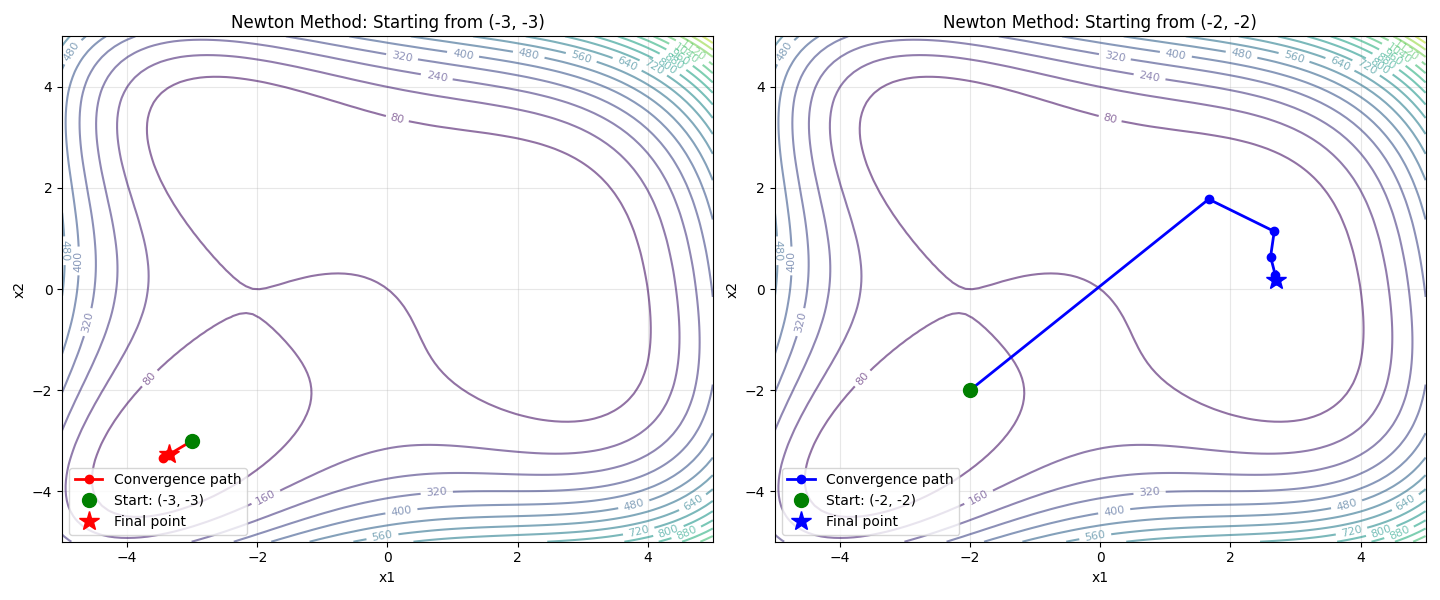
\includegraphics[width=0.8\textwidth]{Figure_1.png}
    \caption{Newton's method convergence paths from different initial points. The red path shows convergence from $(-3, -3)$ to the global optimum, while the blue path shows convergence from $(-2, -2)$ to a local optimum.}
    \label{fig:newton_convergence}
\end{figure}

Figure \ref{fig:newton_convergence} visually demonstrates the convergence behavior described above, showing how the two different initial points lead to completely different local optima.

\item Figure \ref{fig:water} below illustrates the water network of Newville. The lines are water piplelines numbered from 1 through 11. The arrows on the lines are possible direction(s) of flow of water in these pipelines. The circles are water sources numbered A, B, C. The squares are houses D, E, F, G, H, I. The maximum possible capacity of the water sources are (the sources can operate at less than the
maximum capacity): 
A: 100 Units, B: 100 Units, C: 120 Units.
Demands of water in the houses are:
D: 50 Units, E: 60 Units, F: 40 Units, G: 30 Units, H: 70 Units, I: 40 Units.
Since the houses are at different elevation and the pipes are of different diameter, the cost of transporting water is different in the different pipes. These costs per unit of water are:
Pipe 1: \$2, Pipe 2: \$3, Pipe 3: \$4, Pipe 4: \$2, Pipe 5: \$3, Pipe 6: \$2, Pipe 7: \$4, Pipe 8: \$1, Pipe 9: \$2, Pipe 10: \$4, Pipe 11: \$5, Pipe 12: \$3.
Formulate an LP to minimize the total cost of transporting water so as to meet the water demands of each house. 

\begin{figure}[h!]
    \centering
    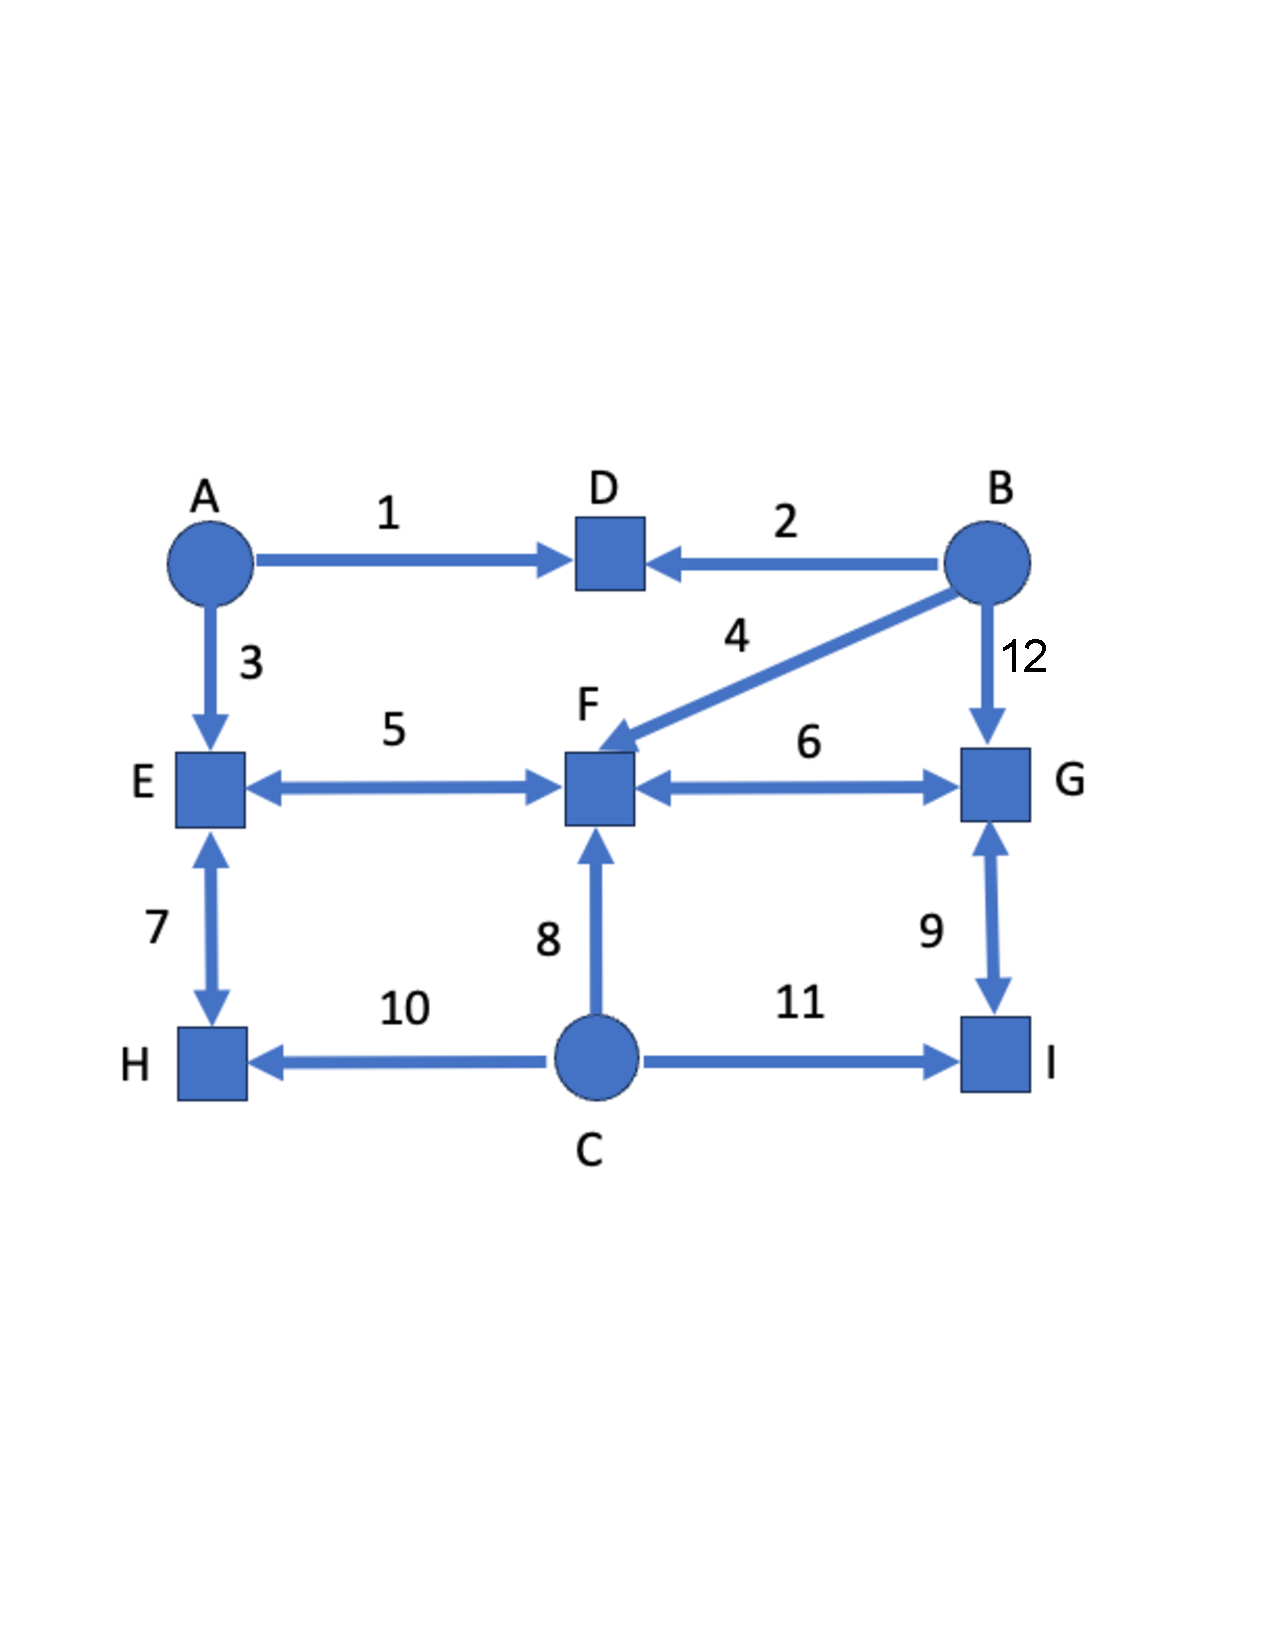
\includegraphics[scale=0.5]{newwaterfig.pdf}
    \caption{Water Network for Question 2}
    \label{fig:water}
\end{figure}

\subsection*{Solution.}

We formulate this water network optimization problem as a minimum cost flow linear programming problem.

\subsubsection*{Decision Variables}
Let $x_i$ denote the flow through pipeline $i$ for $i \in \{1, 2, 3, 4, 5, 6, 7, 8, 9, 10, 11, 12\}$.

For bidirectional pipelines (5, 6, 7, 9), we introduce additional variables for reverse flow:
\begin{itemize}
    \item $x_{-5}$: reverse flow through pipeline 5 (from E to F)
    \item $x_{-6}$: reverse flow through pipeline 6 (from G to F)  
    \item $x_{-7}$: reverse flow through pipeline 7 (from H to E)
    \item $x_{-9}$: reverse flow through pipeline 9 (from I to G)
\end{itemize}

\subsubsection*{Objective Function}
Minimize the total transportation cost:
\begin{align}
\min \quad & 2x_1 + 3x_2 + 4x_3 + 2x_4 + 3x_5 + 2x_6 + 4x_7 + x_8 \\
& + 2x_9 + 4x_{10} + 5x_{11} + 3x_{12} + 3x_{-5} + 2x_{-6} + 4x_{-7} + 2x_{-9}
\end{align}

\subsubsection*{Constraints}

\textbf{Source capacity constraints:}
\begin{align}
x_1 + x_3 &\leq 100 \quad \text{(Source A)} \\
x_2 + x_4 + x_{12} &\leq 100 \quad \text{(Source B)} \\
x_8 + x_{10} + x_{11} &\leq 120 \quad \text{(Source C)}
\end{align}

\textbf{Demand satisfaction constraints:}
\begin{align}
x_1 + x_2 &\geq 50 \quad \text{(House D)} \\
x_3 + x_7 + x_{-5} - x_5 - x_{-7} &\geq 60 \quad \text{(House E)} \\
x_4 + x_5 + x_6 + x_8 - x_{-5} - x_{-6} &\geq 40 \quad \text{(House F)} \\
x_{-6} + x_9 + x_{12} - x_6 - x_{-9} &\geq 30 \quad \text{(House G)} \\
x_{-7} + x_{10} - x_7 &\geq 70 \quad \text{(House H)} \\
x_{-9} + x_{11} - x_9 &\geq 40 \quad \text{(House I)}
\end{align}

\textbf{Non-negativity constraints:}
\begin{align}
x_i \geq 0 \quad \forall i \in \{1, 2, 3, 4, 5, 6, 7, 8, 9, 10, 11, 12, -5, -6, -7, -9\}
\end{align}

\subsubsection*{Optimal Solution}

Using Gurobi optimizer, we obtain the following optimal solution:

\begin{center}
\begin{tabular}{|c|c|c|c|}
\hline
Pipeline & Flow & Pipeline & Flow \\
\hline
$x_1$ & 50.0 & $x_7$ & 0.0 \\
$x_2$ & 0.0 & $x_8$ & 50.0 \\
$x_3$ & 50.0 & $x_9$ & 0.0 \\
$x_4$ & 0.0 & $x_{10}$ & 70.0 \\
$x_5$ & 0.0 & $x_{11}$ & 0.0 \\
$x_6$ & 0.0 & $x_{12}$ & 70.0 \\
\hline
$x_{-5}$ & 10.0 & $x_{-7}$ & 0.0 \\
$x_{-6}$ & 0.0 & $x_{-9}$ & 40.0 \\
\hline
\end{tabular}
\end{center}

\textbf{Optimal total cost:} \$950

\subsubsection*{Flow Analysis}

The optimal solution can be interpreted as follows:

\begin{itemize}
    \item \textbf{Source A (100 units used):} Supplies 50 units to house D via pipeline 1, and 50 units to house E via pipeline 3
    \item \textbf{Source B (70 units used):} Supplies 70 units to house G via pipeline 12
    \item \textbf{Source C (120 units used):} Supplies 50 units to house F via pipeline 8, and 70 units to house H via pipeline 10
    \item \textbf{Internal redistribution:} 
        \begin{itemize}
            \item House E sends 10 units to house F via reverse pipeline 5 (flow $x_{-5} = 10$)
            \item House G sends 40 units to house I via reverse pipeline 9 (flow $x_{-9} = 40$)
        \end{itemize}
\end{itemize}

\subsubsection*{Demand Verification}

Let us verify that all demands are satisfied:
\begin{itemize}
    \item House D: $x_1 + x_2 = 50 + 0 = 50$ $\surd$
    \item House E: $x_3 + x_7 + x_{-5} - x_5 - x_{-7} = 50 + 0 + 10 - 0 - 0 = 60$ $\surd$  
    \item House F: $x_4 + x_5 + x_6 + x_8 - x_{-5} - x_{-6} = 0 + 0 + 0 + 50 - 10 - 0 = 40$ $\surd$
    \item House G: $x_{-6} + x_9 + x_{12} - x_6 - x_{-9} = 0 + 0 + 70 - 0 - 40 = 30$ $\surd$
    \item House H: $x_{-7} + x_{10} - x_7 = 0 + 70 - 0 = 70$ $\surd$
    \item House I: $x_{-9} + x_{11} - x_9 = 40 + 0 - 0 = 40$ $\surd$
\end{itemize}

All constraints are satisfied and the minimum cost to meet all water demands is \$950.

	\newpage
	\item Consider the following electric power network shown in Figure \ref{fig:power}. This network is taken from a real-world electric power system. Electricity generators are located at nodes 1, 3, and 5 and producing $p_1, p_2, p_3$ amounts of electricity, respectively. Electricity loads are located at nodes 2, 4, and 6 and are consuming $d_1, d_2, d_3$ amounts of electricity, respectively. 
	
	The demand is fixed and given as $d_1 = 120, \; d_2 = 95, \; d_3 = 105$.
	
	Each generator $i$'s production must be within an upper and a lower bound as $p_i^{min}\le p_i \le p_i^{max}$. The bounds are given as $p_1^{\text{min}} = 20, \; p_1^{\text{max}} = 270,\; p_2^{\text{min}} = 20,\; p_2^{\text{max}} = 250, \; p_3^{\text{min}} = 10, \; p_3^{\text{max}} = 300$. 
	
	The flow limits over lines are given as $f_{12}^{\text{max}} = 100, f_{23}^{\text{max}} = 120, f_{34}^{\text{max}} = 50, f_{45}^{\text{max}} = 90, f_{56}^{\text{max}} = 60, f_{61}^{\text{max}} = 50$. 
	
	The line parameters are given as $B_{12} = 11.6, \; B_{23} = 5.9, \; B_{34} = 13.7, \; B_{45} = 9.8, \; B_{56} = 5.6, \; B_{61} = 10.5$. The unit generation costs are given as $c_1 = 10, c_2 = 5, c_3 = 8$.
	
	\begin{enumerate}
		\item Formulate the power system scheduling problem using the model discussed in Lecture 2. 
		
		\item Implement and solve the model using CVXPY. Write down the optimal solution.
		
		\item Find the electricity prices for demand at nodes 2, 4, 6. To do this, use the command \textsf{constraints[0].dual\_value} to find the dual variable of \textsf{constraints[0]}. Hint: Recall the electricity price at node $i$ is the dual variable for the flow conservation constraint at node $i$.
	\end{enumerate}  
	\begin{figure}[h!]
		\centering
		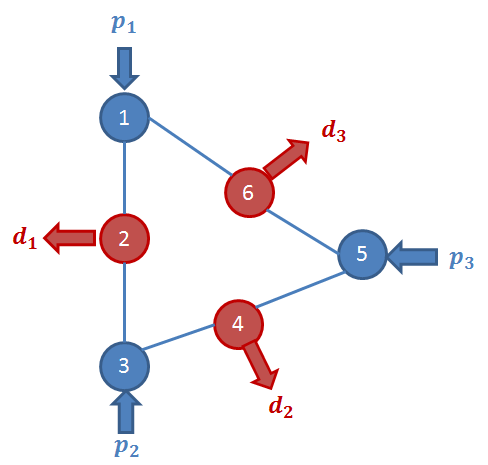
\includegraphics[scale=0.7]{HW5power.png}
		\caption{Electric network for Question 3.}
		\label{fig:power}
	\end{figure}

\subsection*{Solution.}

\subsubsection*{(a) Problem Formulation}

We formulate this as a DC power flow optimization problem. The decision variables are:
\begin{itemize}
    \item $p_i$: power generation at generator node $i$ for $i \in \{1, 3, 5\}$
    \item $f_{ij}$: power flow on line $(i,j)$ for lines $(1,2), (2,3), (3,4), (4,5), (5,6), (6,1)$
    \item $\theta_i$: voltage phase angle at node $i$ for $i \in \{1, 2, 3, 4, 5, 6\}$
\end{itemize}

\textbf{Objective Function:}
Minimize the total generation cost:
\begin{align}
\min \quad 10p_1 + 5p_3 + 8p_5
\end{align}

\textbf{Constraints:}

\emph{Generation bounds:}
\begin{align}
20 &\leq p_1 \leq 270 \\
20 &\leq p_3 \leq 250 \\
10 &\leq p_5 \leq 300
\end{align}

\emph{Line flow limits:}
\begin{align}
-100 &\leq f_{12} \leq 100 \\
-120 &\leq f_{23} \leq 120 \\
-50 &\leq f_{34} \leq 50 \\
-90 &\leq f_{45} \leq 90 \\
-60 &\leq f_{56} \leq 60 \\
-50 &\leq f_{61} \leq 50
\end{align}

\emph{DC power flow equations:}
\begin{align}
f_{12} &= 11.6(\theta_1 - \theta_2) \\
f_{23} &= 5.9(\theta_2 - \theta_3) \\
f_{34} &= 13.7(\theta_3 - \theta_4) \\
f_{45} &= 9.8(\theta_4 - \theta_5) \\
f_{56} &= 5.6(\theta_5 - \theta_6) \\
f_{61} &= 10.5(\theta_6 - \theta_1)
\end{align}

\emph{Power balance at each node:}
\begin{align}
\text{Node 1:} \quad p_1 &= f_{12} - f_{61} \\
\text{Node 2:} \quad -120 &= f_{23} - f_{12} \\
\text{Node 3:} \quad p_3 &= f_{34} - f_{23} \\
\text{Node 4:} \quad -95 &= f_{45} - f_{34} \\
\text{Node 5:} \quad p_5 &= f_{56} - f_{45} \\
\text{Node 6:} \quad -105 &= f_{61} - f_{56}
\end{align}

\emph{Reference node:}
\begin{align}
\theta_1 = 0
\end{align}

\subsubsection*{(b) Optimal Solution}

Using Gurobi optimizer, we obtain the following optimal solution:

\textbf{Generation (MW):}
\begin{align}
p_1^* &= 103.09 \text{ MW} \\
p_3^* &= 111.91 \text{ MW} \\
p_5^* &= 105.00 \text{ MW}
\end{align}

\textbf{Line flows (MW):}
\begin{align}
f_{12}^* &= 58.09 \text{ MW} \\
f_{23}^* &= -61.91 \text{ MW} \\
f_{34}^* &= 50.00 \text{ MW} \\
f_{45}^* &= -45.00 \text{ MW} \\
f_{56}^* &= 60.00 \text{ MW} \\
f_{61}^* &= -45.00 \text{ MW}
\end{align}

\textbf{Voltage phase angles (radians):}
\begin{align}
\theta_1^* &= 0.0000 \\
\theta_2^* &= -5.0075 \\
\theta_3^* &= 5.4864 \\
\theta_4^* &= 1.8367 \\
\theta_5^* &= 6.4286 \\
\theta_6^* &= -4.2857
\end{align}

\textbf{Optimal total cost:} \$2430.43

\subsubsection*{(c) Electricity Prices}

The electricity prices at demand nodes are the dual variables of the power balance constraints:

\begin{itemize}
    \item \textbf{Node 2:} \$8.31/MWh
    \item \textbf{Node 4:} \$10.00/MWh  
    \item \textbf{Node 6:} \$11.86/MWh
\end{itemize}

These prices reflect the marginal cost of serving an additional unit of demand at each location. Node 6 has the highest price (\$11.86/MWh) due to transmission constraints, while Node 2 has the lowest price (\$8.31/MWh) as it is closest to the low-cost generator at Node 3.

\end{enumerate}

\end{document}